\section{Results}
\label{sec:results}

% BIFURCATION_TABLE

The analytical derivations, extended parameter sweeps and secondary policy
experiments are reported in the Supplementary Material. The main text keeps
the nonlinear transitions and the global basin result that organise them.

\subsection{When certification is needed}
\label{sec:reciprocity}

Consider an unbadged population that plays \CS{}: open safely, then mirror. A
rare \CAS{} mutant opens unsafely and retains its initial lead even after the
resident retaliates. It earns $61.63$ against the resident's $59.00$, at the
cost of $4.78$ additional unsafe actions.

\begin{proposition}[Reciprocity threshold]
\label{prop:reciprocity}
At zero assortment, the first-striker's advantage vanishes at
\begin{equation}
\label{eq:LR}
L_R=\frac{A(\CAS,\CS)-A(\CS,\CS)}
          {M(\CAS,\CS)-M(\CS,\CS)}=0.551.
\end{equation}
For the canonical safe resident, its joint invasion advantage is
\begin{equation}
\label{eq:jointfirststrike}
\Delta(L,r)=2.631-34.431r-(4.78+4.22r)L.
\end{equation}
Thus $L_R$ and
\begin{equation}
\label{eq:rdagger}
r^{\dagger}=\frac{A(\CAS,\CS)-A(\CS,\CS)}
 {A(\CAS,\CS)-A(\CAS,\CAS)}=0.076
\end{equation}
are intercepts of one boundary, not independent bounds. At $r=0$, no
unbadged population sustains safe play for $L<L_R$.
\end{proposition}

Assortment makes an aggressive mutant meet its own aggression and removes the
opening advantage above $r^{\dagger}$. Below the joint boundary, however,
something outside the race must distinguish partners before the first move;
this is the role of a badge. Figure~\ref{fig:handshake} shows both the local
exploit and its population consequence.

At $L=0$ and $r=0$, the unbadged world consequently runs at unsafe frequency
$1.000$. At the baseline $r=0.1$, the four unbadged residents whose realised
conduct is \CS{} can resist the first-striker, explaining why the uncertified
face found below is safe despite zero liability. Identity is therefore most
valuable where neither attribution nor interaction structure closes the
first-move advantage; once $L>L_R$, liability performs the same deterrent task
without a credential layer.

\begin{figure}[pos=t]
\centering
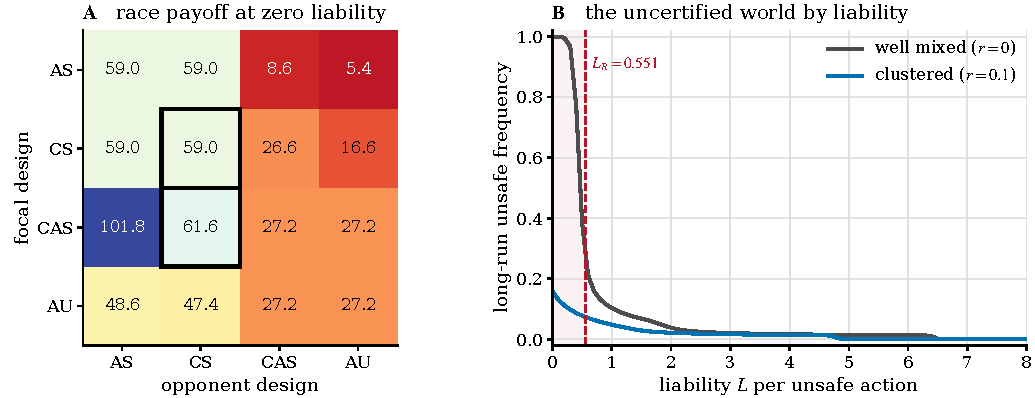
\includegraphics[width=\linewidth]{figures/fig02_handshake.pdf}
\caption{\textbf{Why identity is needed.} \textbf{(A)} Private race payoff at
$L=0$; boxed cells mark the first-move exploit. \textbf{(B)} Unsafe frequency
of the unbadged world against liability. The shaded region lies below
$L_R=0.551$; assortment above $r^{\dagger}=0.076$ partly restores safe
reciprocity.}
\label{fig:handshake}
\end{figure}

\subsection{Forgery tolerance and the detection limit}
\label{sec:spoof}

A certified club $(\mathsf{G},u,v)$ plays $u$ after a passed check and $v$
otherwise. A forger pays $\kappa_f$ rather than $\kappa_g$ and passes with
probability $\sigma$.

\begin{proposition}[Spoof threshold]
\label{prop:spoof}
For an unconditional forger $(\mathsf{F},w,w)$ against the club in a
well-mixed population, the threshold is
\begin{equation}
\label{eq:sigmastar}
\sigma^{*}=\frac{P(u,u)-P(w,v)-\kappa_g+\kappa_f+\rho}
 {P(w,u)-P(w,v)+\rho},\qquad P=A-LM.
\end{equation}
When the denominator is positive, the club resists below $\sigma^{*}$; when it
is negative the inequality reverses; when it vanishes the invasion advantage
is independent of $\sigma$.
\end{proposition}

The in-group conduct enters Equation~\eqref{eq:sigmastar} through both member
payoff and impostor extraction. Consequently, the reciprocating club
$(\mathsf{G},\CS,\CAS)$ tolerates $\sigma^{*}=0.866$ when well mixed and
$0.962$ at $r=0.1$, whereas an unconditionally trusting club tolerates only
$0.400$ and $0.444$. The $2.17$ ratio is unchanged: membership conduct, not
goodwill, is the security parameter.

The sign condition in Proposition~\ref{prop:spoof} separates exclusionary from
gentle clubs. Harsh out-group conduct makes passing valuable to an impostor and
creates a positive, finite invasion threshold. If $u=v$, a badge changes no
conduct; without a fine, the forger's advantage is simply the dues it avoids
and is independent of verification quality. This connects the local spoof
threshold to the global entry-barrier result below.

Assortment penalises an exploiter's self-encounters but scarcely affects a
behavioural mimic. Their invasion curves cross at $r=0.077$ and the exploiter
is excluded entirely above $r=0.134$ (Figure~\ref{fig:invasion}). At the
intersection, two independent transversal eigenvalues vanish and two
transcritical edge bifurcations coincide. The club vertex remains non-hyperbolic
because genuine designs that differ only in unused out-group conduct are
payoff-equivalent; the codimension-two claim concerns the two invading edges,
not a new normal form for the full vertex.

\begin{figure}[pos=t]
\centering
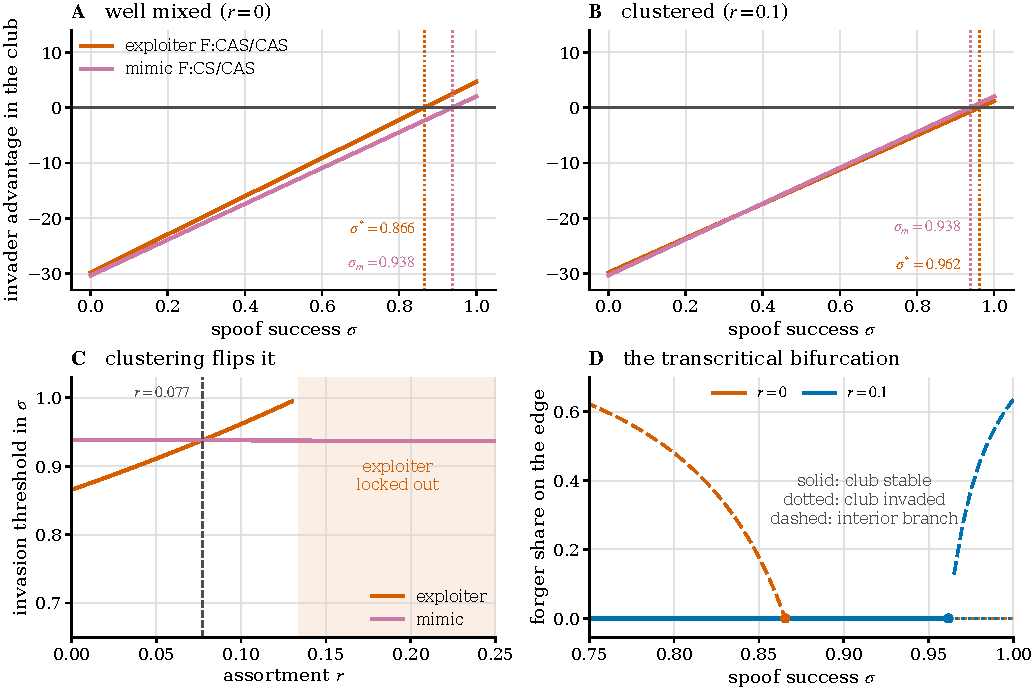
\includegraphics[width=\linewidth]{figures/fig03_invasion.pdf}
\caption{\textbf{Invasion and edge bifurcation.} Invader advantages when
\textbf{(A)} well mixed and \textbf{(B)} at $r=0.1$; \textbf{(C)} thresholds
against assortment; \textbf{(D)} the transcritical exchange on the
club--exploiter edge. Assortment removes the visible exploiter before the
behavioural mimic.}
\label{fig:invasion}
\end{figure}

\paragraph{Detection and penalties.}
Setting the same invasion advantage to zero for the fine gives a hard limit on
enforcement.

\begin{proposition}[Becker limit of attestation]
\label{prop:fines}
The break-even fine in a well-mixed population is
\begin{equation}
\label{eq:rhostar}
\rho^{*}(\sigma)=
\frac{\sigma[P(w,u)-P(w,v)]-[P(u,u)-P(w,v)]+\kappa_g-\kappa_f}
 {1-\sigma},
\end{equation}
which diverges as $\sigma\to1$ whenever full-pass exploitation beats honest
membership. Where the club already resists, the smallest feasible fine is
$\max\{0,\rho^{*}\}$.
\end{proposition}

The required fine rises from $11.9$ at $\sigma=0.90$ to $428.6$ at $0.99$ in
the well-mixed case. The pole remains under assortment because the expected
penalty is $(1-\sigma)\rho$: sanctions cannot replace a detection event that
never occurs. Dues weaken the club, whereas a higher forgery cost burdens the
impostor. Figure~\ref{fig:instruments} summarises these comparative statics;
the full dues--fine sweep is Supplementary Table S1.

In standard enforcement, detection effort and penalty size may be purchased as
substitutes~\citep{becker1968crime,polinsky2000economic}. Here $\sigma$ is fixed
by the verification technology, so a regulator cannot buy a larger expected
penalty once detection disappears. The fine is imposed by an authority rather
than voluntarily by peers and therefore avoids the second-order free-rider
problem of costly punishment~\citep{szolnoki2017second}; its binding constraint
is technological detection.

\begin{figure}[pos=t]
\centering
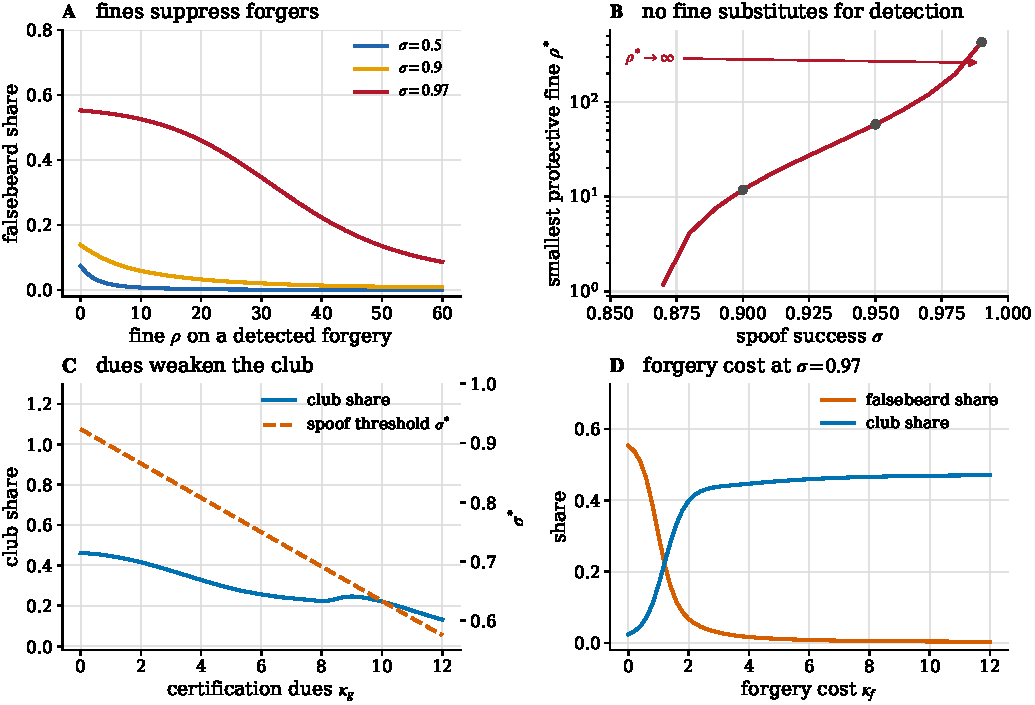
\includegraphics[width=\linewidth]{figures/fig06_instruments.pdf}
\caption{\textbf{Enforcement instruments.} \textbf{(A)} Fines suppress
forgers only when detection is informative. \textbf{(B)} The protective fine
diverges as $\sigma\to1$. \textbf{(C)} Certification dues weaken the club.
\textbf{(D)} A direct forgery cost instead burdens the impostor.}
\label{fig:instruments}
\end{figure}

\subsection{A club must nucleate before it can resist}
\label{sec:nucleation}

The preceding thresholds condition on a club already being present.
Verification alone cannot create one.

\begin{proposition}[Badge futility]
\label{prop:futility}
Against a resident whose conduct does not condition on badges, a certified
design earns exactly its unbadged twin's payoff minus $\kappa_g$, for every
$\sigma$, $\rho$ and $L$. Hence no costly badge invades at $r=0$ unless its
unbadged twin already can.
\end{proposition}

Assortment supplies the self-encounters that let the signal be read.

\begin{proposition}[Nucleation threshold]
\label{prop:nucleation}
Against $(\mathsf{N},w,w)$, a club $(\mathsf{G},u,v)$ with
$P(u,u)>P(v,w)$ invades exactly when
\begin{equation}
\label{eq:rstar}
r>r^{*}=\frac{P(w,w)-P(v,w)+\kappa_g}{P(u,u)-P(v,w)}=0.063
\end{equation}
at the baseline. If the denominator is negative the inequality reverses; if it
vanishes the club cannot invade at any assortment.
\end{proposition}

Thus verification quality and assortment are not substitutes: $\sigma$ does
not appear in Equation~\eqref{eq:rstar}. Moreover, keeping a club is easier
than rebuilding it. At $r=0$ a collapsed club cannot re-enter either forgery
or anarchy at any verification quality, producing the hysteresis-like
asymmetry in Figure~\ref{fig:nucleation}.

The resident matters. Against the anarchic $(\mathsf{N},\CAS,\CAS)$ resident,
self-encounters expose a nascent club to its safe in-group payoff and make
assortment constructive. Against the already safe
$(\mathsf{N},\CS,\CS)$ resident, the denominator in
Equation~\eqref{eq:rstar} is negative and the club invades only below
$r=0.240$: assortment instead protects the incumbent safe regime. Formation
and persistence are distinct invasion problems, not two readings of one
threshold.

\begin{figure}[pos=t]
\centering
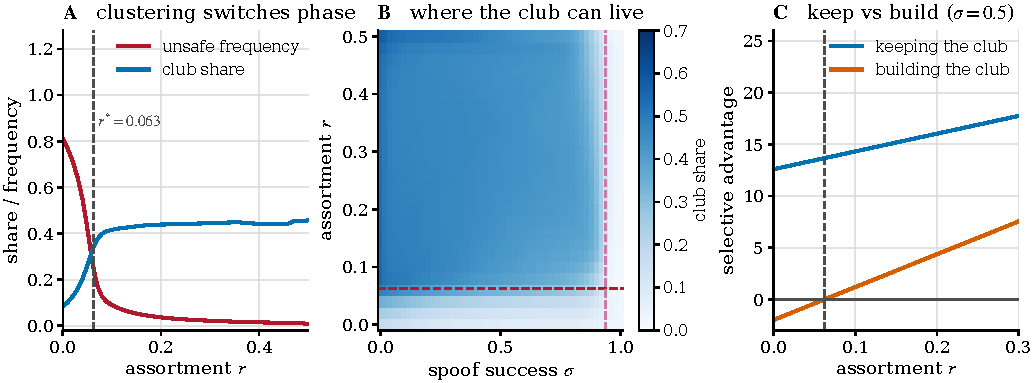
\includegraphics[width=\linewidth]{figures/fig05_nucleation.pdf}
\caption{\textbf{Club nucleation.} \textbf{(A)} The club appears at
$r^{*}=0.063$. \textbf{(B)} Its viable region is bounded by nucleation and
mimicry thresholds. \textbf{(C)} The advantage of retaining a club exceeds
the advantage of rebuilding one after collapse.}
\label{fig:nucleation}
\end{figure}

\subsection{Hollow collapse precedes unsafe conduct}
\label{sec:mimicry}

An exploiter is not the first threat. A behavioural mimic
$(\mathsf{F},u,v)$ copies club conduct and free-rides only on the dues.

\begin{proposition}[Mimicry threshold]
\label{prop:mimicry}
When $r=0$, the mimic invades when
\begin{equation}
\label{eq:sigmam}
\sigma>\sigma_m=1-\frac{\kappa_g-\kappa_f}
 {P(u,u)-P(u,v)+\rho}=0.938.
\end{equation}
At $r=0.1$ the exact advantage is quadratic in $\sigma$ and its admissible
root is $0.9377$, below the exploiter threshold $0.9617$.
\end{proposition}

At $\sigma=0.96$, inside this window, forgers hold $0.54$ of the population
and the club only $0.04$, yet unsafe frequency falls to $0.063$. Attestation
integrity is $0.07$: conduct looks sound after the credential has become
nearly meaningless. The behavioural value of a passed badge becomes negative
even earlier, at $\sigma=0.57$, because passing increasingly selects the
partners most able to exploit it (Figure~\ref{fig:cliff}). Real-time screening
and retrospective fines improve integrity through distinct, complementary
channels, but unsafe frequency alone barely distinguishes them; the full
$2\times2$ experiment is Supplementary Figure S1.

This ordering explains why better interaction structure can hide rather than
remove residual risk. Assortment raises the exploiter threshold from $0.866$
to $1$ because exploiters suffer in self-play, while the mimic threshold moves
by only $0.001$. Beyond $r=0.134$, the remaining sampled invasion route is an
agent that behaves correctly. Conduct monitoring then reports success exactly
where the identity signal has become least informative.

\begin{figure}[pos=t]
\centering
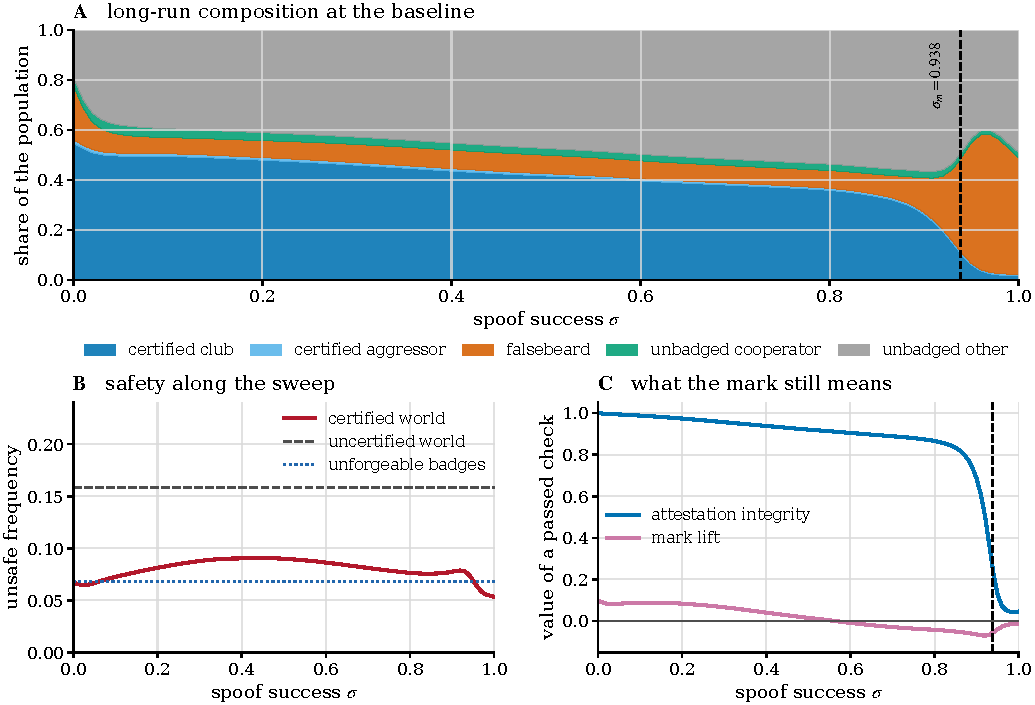
\includegraphics[width=\linewidth]{figures/fig04_cliff.pdf}
\caption{\textbf{Hollow collapse.} \textbf{(A)} Composition against spoof
success. \textbf{(B)} Unsafe frequency with forgeable, unforgeable and absent
badges. \textbf{(C)} Attestation integrity collapses at $\sigma_m$, while the
behavioural value of a passed badge becomes negative at $\sigma=0.57$.}
\label{fig:cliff}
\end{figure}

\subsection{Multistability turns protection into an entry barrier}
\label{sec:exclusion}

The finite-population process describes recurrent mutation and fixation. The
replicator flow instead asks where an arbitrary composition settles, and its
answer is not unique.

\begin{observation}[Dominant two-face split and a targeted unsafe rest face, numerical]
\label{prop:bistable}
At the baseline, $38.8\%$ of $20\,000$ uniform Dirichlet starts converge to an
entirely badged rest state and $61.2\%$ to an entirely unbadged one (Wilson
$95\%$ interval $[38.2,39.5]$ for the first share). Every sampled endpoint is
invasion-resistant and has unsafe frequency below $10^{-13}$. A targeted start
with mass $0.70$ on $(\mathsf{F},\AU,\AU)$ instead reaches an invasion-resistant
mixed rest state with $U=1.000$ and badged mass $0.937$; all 64 recorded
full-dimensional perturbations do likewise. This probe establishes local
numerical robustness, not its basin volume or a third isolated attractor.
\end{observation}

The two dominant limit sets are faces rather than isolated equilibria. Within
a certified population, out-group conduct is unused and neutral; within an
uncertified population, in-group conduct is unused. Each run therefore retains
a memory of its transient composition. The $38.8\%$ share belongs to the
chosen start measure and is not a property of the flow itself.

More specifically, genuine designs with the same realised in-group conduct
earn the same payoff on the certified face, and unbadged designs with the same
realised out-group conduct do likewise. The attracting portions of these faces
are cut out by the requirement that no absent design have positive growth;
the entire faces are not uniformly attracting. Calling the outcome ``two
equilibria'' would therefore erase both the neutral directions and the
continuum of endpoints reached by the $20\,000$ runs.

\begin{corollary}[No safety dividend on the dominant safe faces]
\label{cor:dues}
The certified and uncertified dominant faces are both safe, with social payoff
$57.0$ and $59.0$. Conditional on either settled regime, certification buys no
additional safety and costs exactly $\kappa_g=2$.
\end{corollary}

This does not contradict the small-mutation result, under which certification
reduces unsafe frequency from $0.159$ to $0.090$. It reduces harm while the
market is displaced from safety and returns, rather than the harm of either
settled face. Certification buys robustness, not a lower stationary level.

\begin{proposition}[The entry barrier]
\label{prop:exclusion}
A compliant unbadged entrant plays the club's own in-group conduct towards
everyone. Against $(\mathsf{G},\CS,\CAS)$ it earns $26.64$ where a member nets
$57.00$, a well-mixed penalty of $30.36$, and the encounter has unsafe
frequency $0.461$. Against the gentle club $(\mathsf{G},\CS,\CS)$ the penalty
is $-2.00$ and the encounter is safe.
\end{proposition}

The barrier is selection pressure, not a fee that an outsider is forbidden to
pay. Table~\ref{tab:outgroup} shows that the two gentle policies impose no
barrier but have spoof threshold zero; the two harsh policies resist forgery
and dominate under rare mutation. Excludability is therefore the mechanism
that makes costly membership evolutionarily distinct.

This mechanism differs from parochial altruism maintained by group
competition~\citep{choi2007parochial}. No group-level contest occurs here.
Harsh out-group conduct instead makes the benefit of the dues excludable and
raises the potential cost of cheating relative to honest acquisition, an
off-equilibrium cost capable of maintaining a costly signal
~\citep{szamado2011cost}.

\begin{table}[pos=t]
\centering
\caption{Out-group conduct jointly determines forgery tolerance and the payoff
penalty imposed on a compliant unbadged entrant.}
\label{tab:outgroup}
\small
\begin{tabular}{lrrrrr}
\toprule
conduct towards & spoof threshold & entry & boundary & club share & certified \\
outsiders & $\sigma^{*}$ & penalty & unsafe & (monomorphic) & basin \\
\midrule
\AS{}  & 0.000 & $-2.00$ & 0.000 & 0.005 & 0.000 \\
\CS{}  & 0.000 & $-2.00$ & 0.000 & 0.020 & 0.000 \\
\CAS{} & 0.962 & $30.36$ & 0.461 & 1.000 & 0.885 \\
\AU{}  & 0.962 & $40.40$ & 0.868 & 1.000 & 0.395 \\
\bottomrule
\end{tabular}
\end{table}

\begin{corollary}[A fine restores the barrier, not the purpose]
\label{cor:rescue}
A fine $\rho=60$ raises a gentle club's spoof threshold from $0$ to $0.923$,
but its equilibrium share remains below $0.032$ in either dynamic.
\end{corollary}

The fine makes forgery unattractive but cannot make a costly gentle club
preferable to its free unbadged twin. Figure~\ref{fig:exclusion} summarises the
basin split, dues-sized equilibrium cost and barrier--resistance trade-off.
Evaluating bilinear observables at a basin-averaged state would instead invent
cross-face encounters and report $U=0.368$ although every averaged endpoint is
safe; observables must be scored within each attractor before basin averaging.

\begin{figure}[pos=t]
\centering
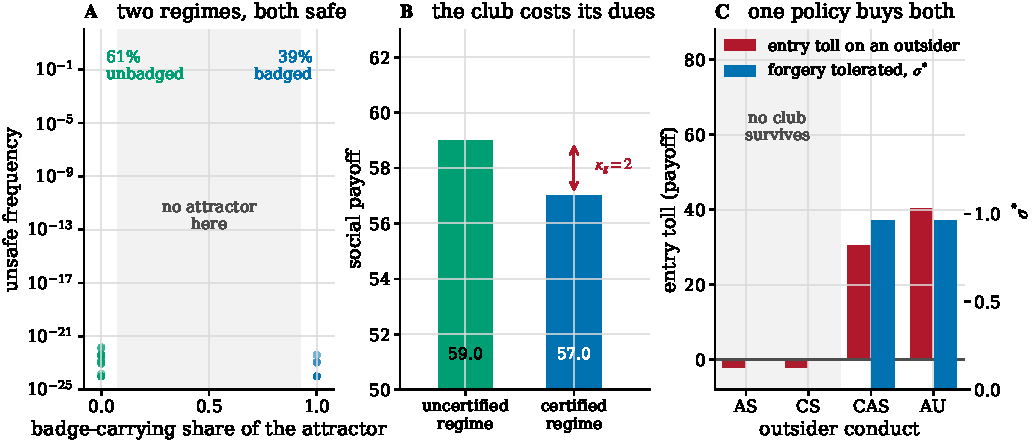
\includegraphics[width=\linewidth]{figures/fig01_exclusion.pdf}
\caption{\textbf{Multistability and exclusion.} \textbf{(A)} Uniform starts
reach certified or uncertified safe faces. \textbf{(B)} The certified face is
poorer by exactly the dues. \textbf{(C)} Forgery tolerance and the entry
penalty rise together across out-group policies.}
\label{fig:exclusion}
\end{figure}

\subsection{Robustness and secondary extensions}
\label{sec:robustness}

The qualitative ordering survives population sizes $50$--$200$, selection
intensities $0.01$--$0.2$ and brute-force checks of every closed-form root.
Finite-population and replicator integrity curves correlate at $0.965$ along
the spoof sweep, although their unsafe-frequency levels differ because they
answer different questions. An alternative reading of the race setback moves
the numerical thresholds but preserves the phase structure. Supplementary
Tables S2--S4 and Figure S3 report these checks. Two secondary extensions are
also separated from the main nonlinear narrative: identity has appreciable
value mainly below the liability threshold, and provider-scoped credentials
make cross-provider harm equal $1-\mathrm{HHI}$ until recognition is federated
(Supplementary Sections S3--S4).

Under the alternative setback reading, for example, $L_R$ moves from $0.551$
to $1.486$, $\sigma^{*}$ from $0.866$ to $0.676$ and $r^{*}$ from $0.063$ to
$0.095$, while the reciprocity, forgery and nucleation phases remain. The main
claims concern these transition mechanisms and their ordering; the position
of a chosen baseline relative to them is specification-dependent.
